\begin{frame}{}
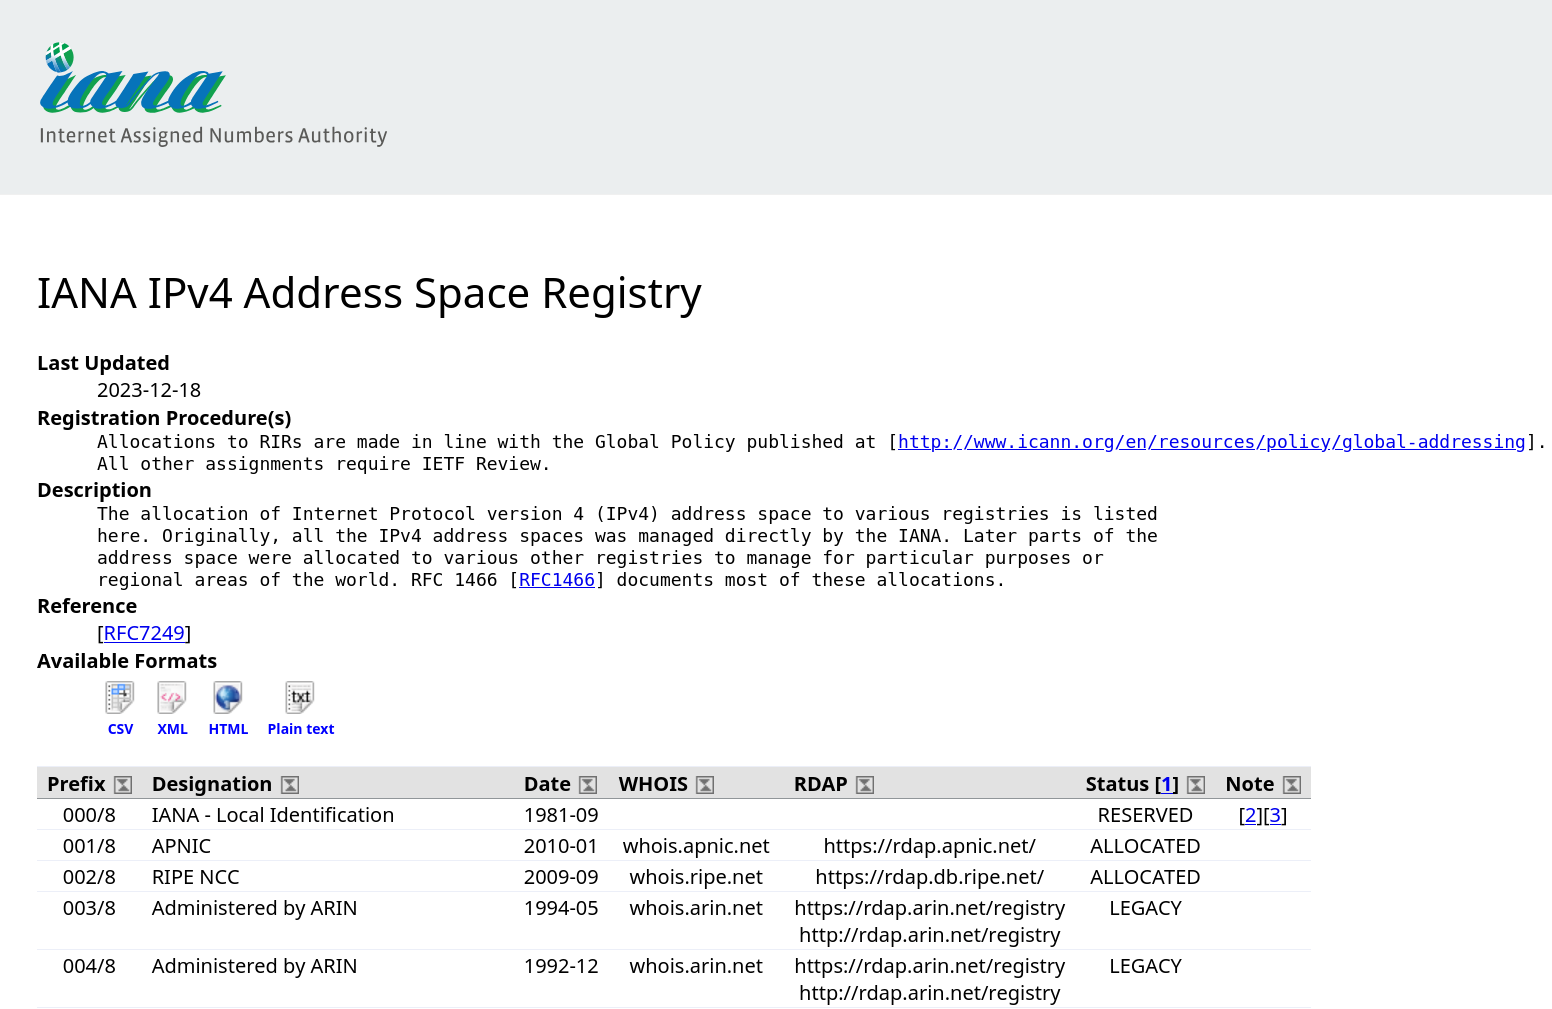
\includegraphics[width=\textwidth]{../arp/iana-registry-screenshot}
\end{frame}

\begin{frame}{}
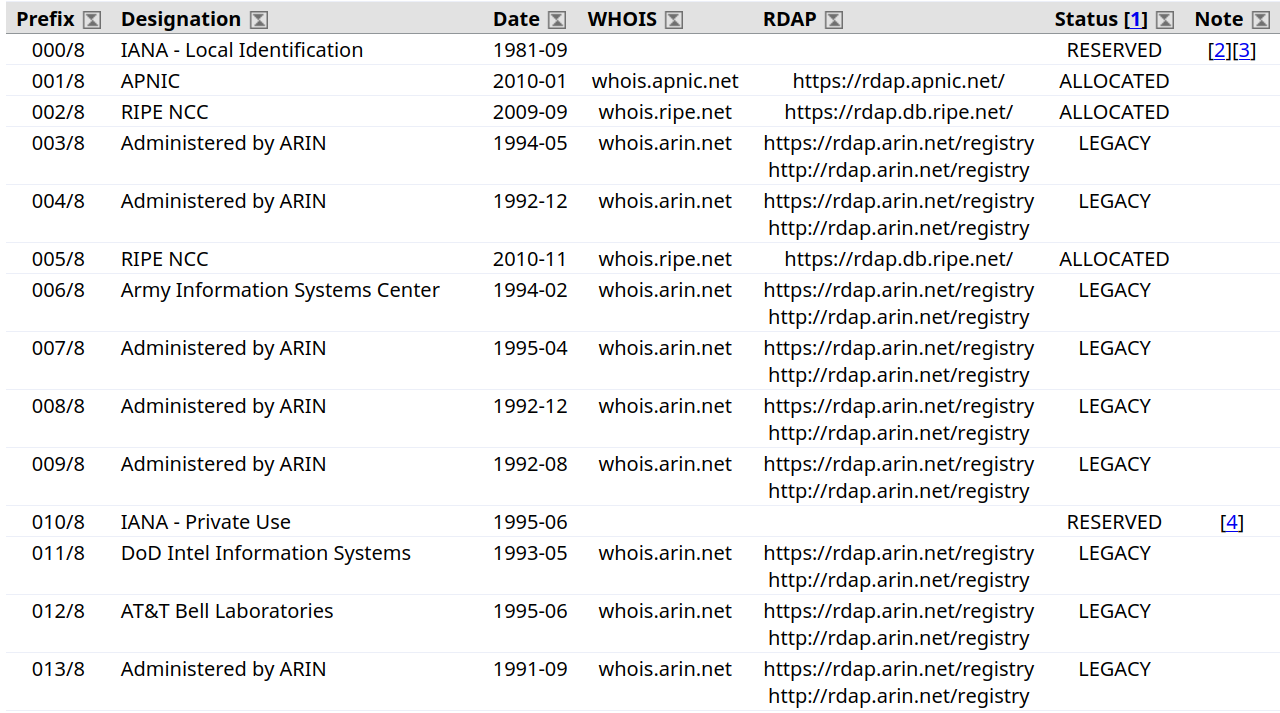
\includegraphics[width=\textwidth]{../arp/iana-ipv4-allocs}
(and 241 more)
\end{frame}

\begin{frame}[fragile]{}
\begin{tikzpicture}
\node (v6 space top) {

\includegraphics[width=8cm]{../arp/iana-v6-addr-top} 
};
\node[anchor=north,font=\Huge,inner sep=1mm] (v6 space ldots) at ([yshift=-1mm]v6 space top.south) {\ldots};
\node[anchor=north] at (v6 space ldots.north) {
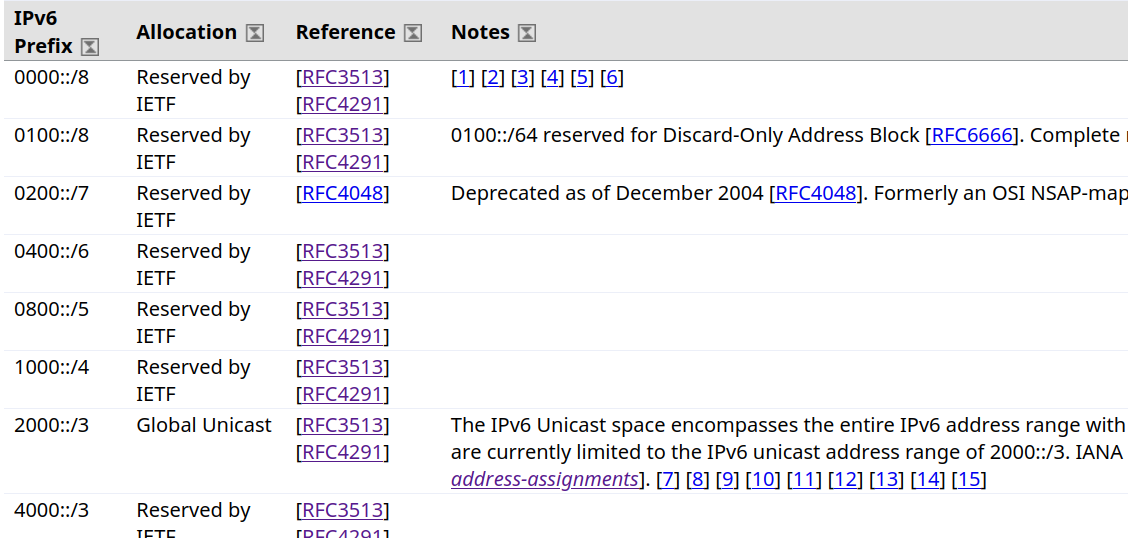
\includegraphics[width=8cm]{../arp/iana-v6-addr-bottom2}
};
\node[anchor=north west] at (v6 space top.north east) {
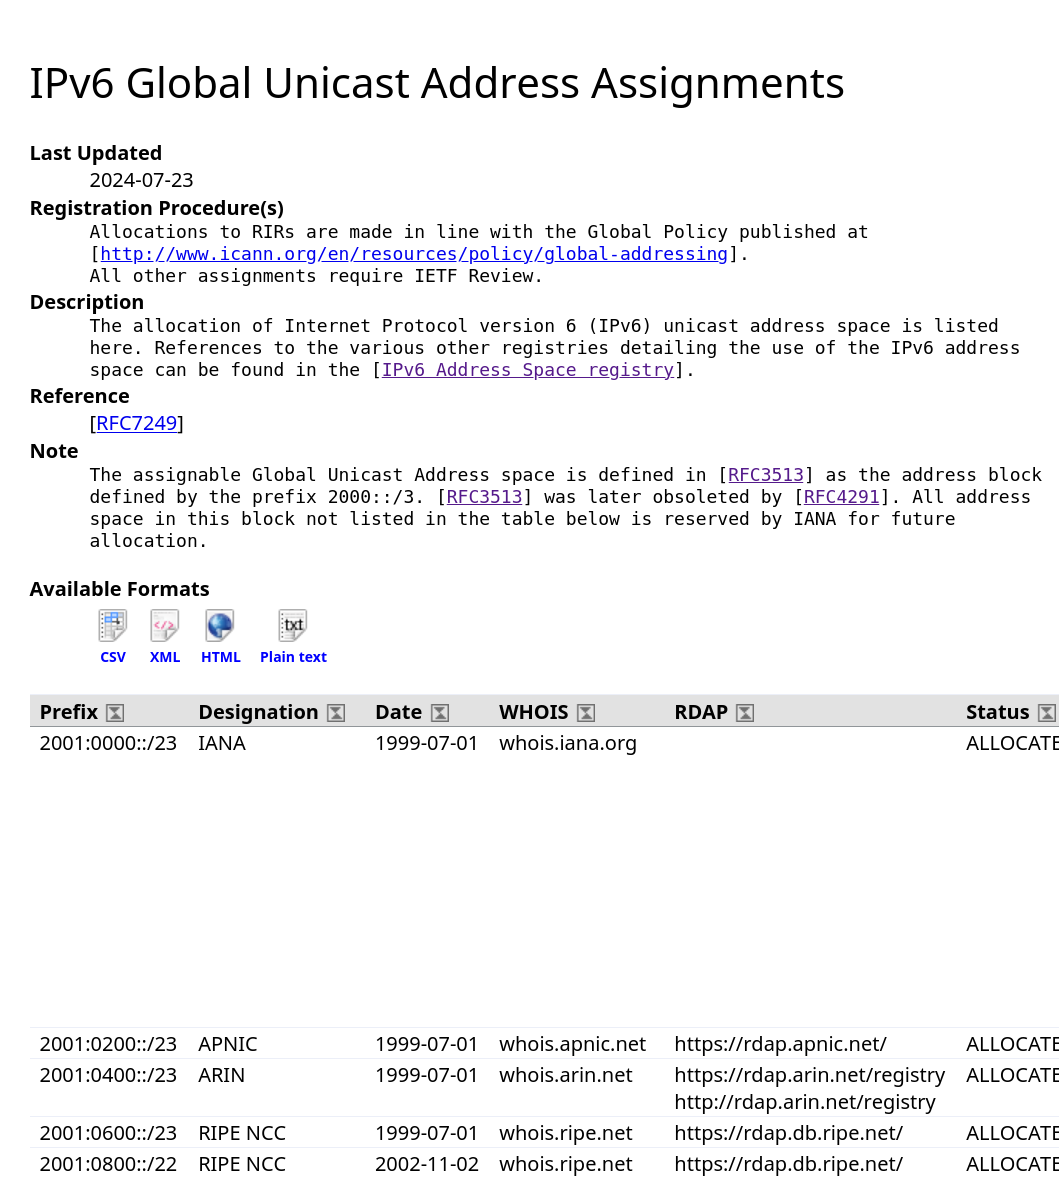
\includegraphics[width=8cm]{../arp/iana-v6-unicast}
};
\end{tikzpicture}
\end{frame}

\begin{frame}{regional internet registries (RIRs)}
\begin{tikzpicture}
\node[inner sep=1mm] (rir) {
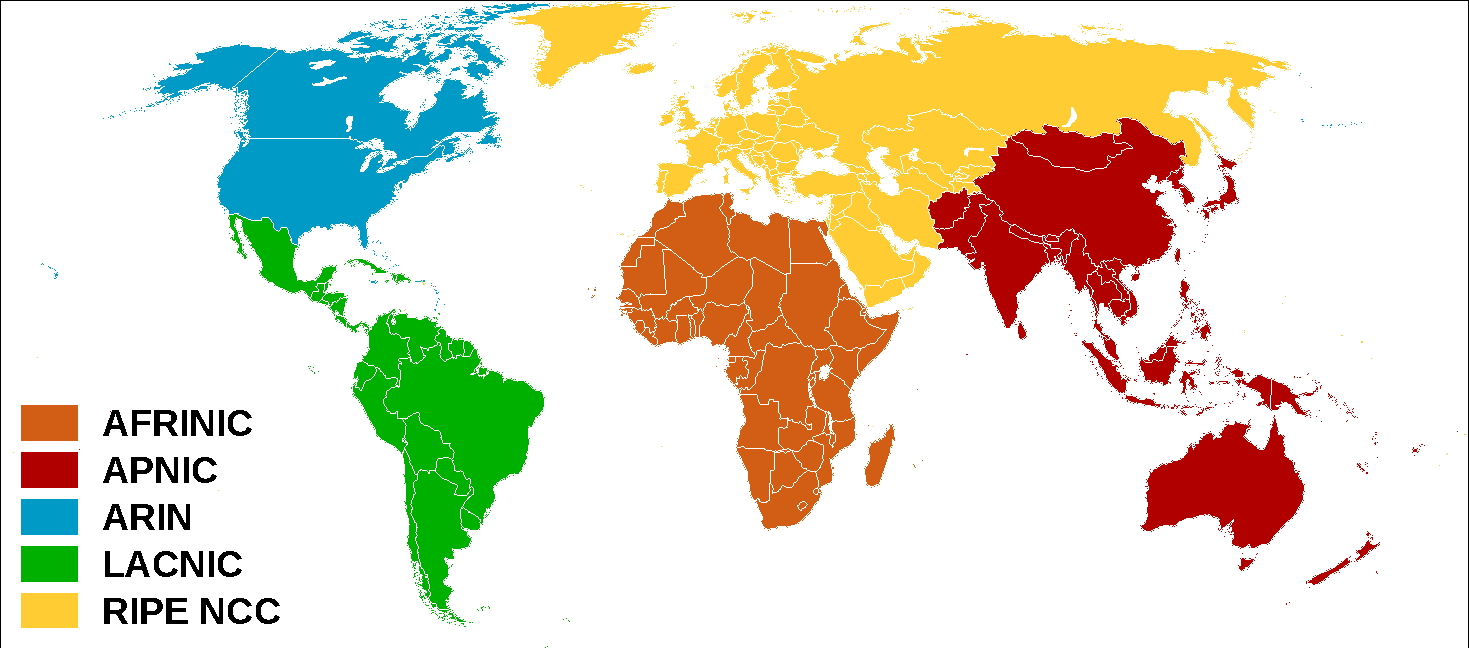
\includegraphics[height=0.35\textheight]{Regional_Internet_Registries_world_map.pdf} 
};
\node[align=left,anchor=north west,font=\scriptsize] at (rir.north east) {
map from Wikimedia Commons, \\
users Dork, Canuckguy et al, S\'emhur, CC-BY-SA 3.0
};
\end{tikzpicture}
\begin{itemize}
\item most useful addresses managed by RIRs
    \begin{itemize}
    \item African Network Information Centre (AFRINIC)
    \item American Registry for Internet Numbers (ARIN)
    \item Asia Pacific Network Information Centre (APNIC)
    \item Latin American and Carribean Network Information Centre (LACNIC)
    \item R\'eseaux IP Europ\'eens Network Coordination Centre (RIPE NCC)
    \end{itemize}
\end{itemize}
\end{frame}

\begin{frame}{RIR suballocations}
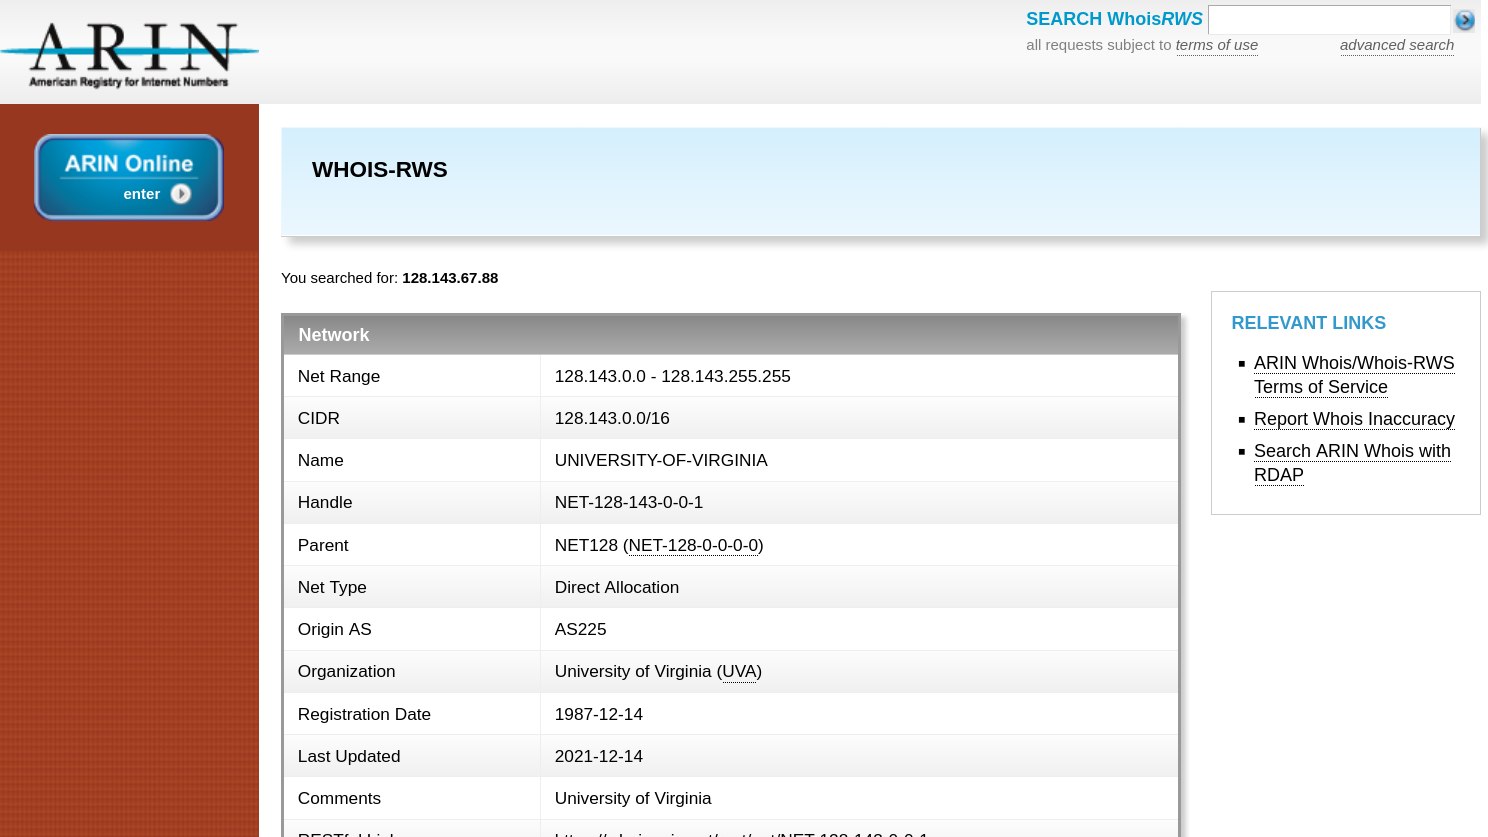
\includegraphics[width=\textwidth]{../arp/arin-whois-virginia}
\end{frame}

\begin{frame}{special IPv4 addresses}

\includegraphics[width=\textwidth]{../arp/iana-special-ipv4-header}
\end{frame}

\begin{frame}{special IPv4 addresses}
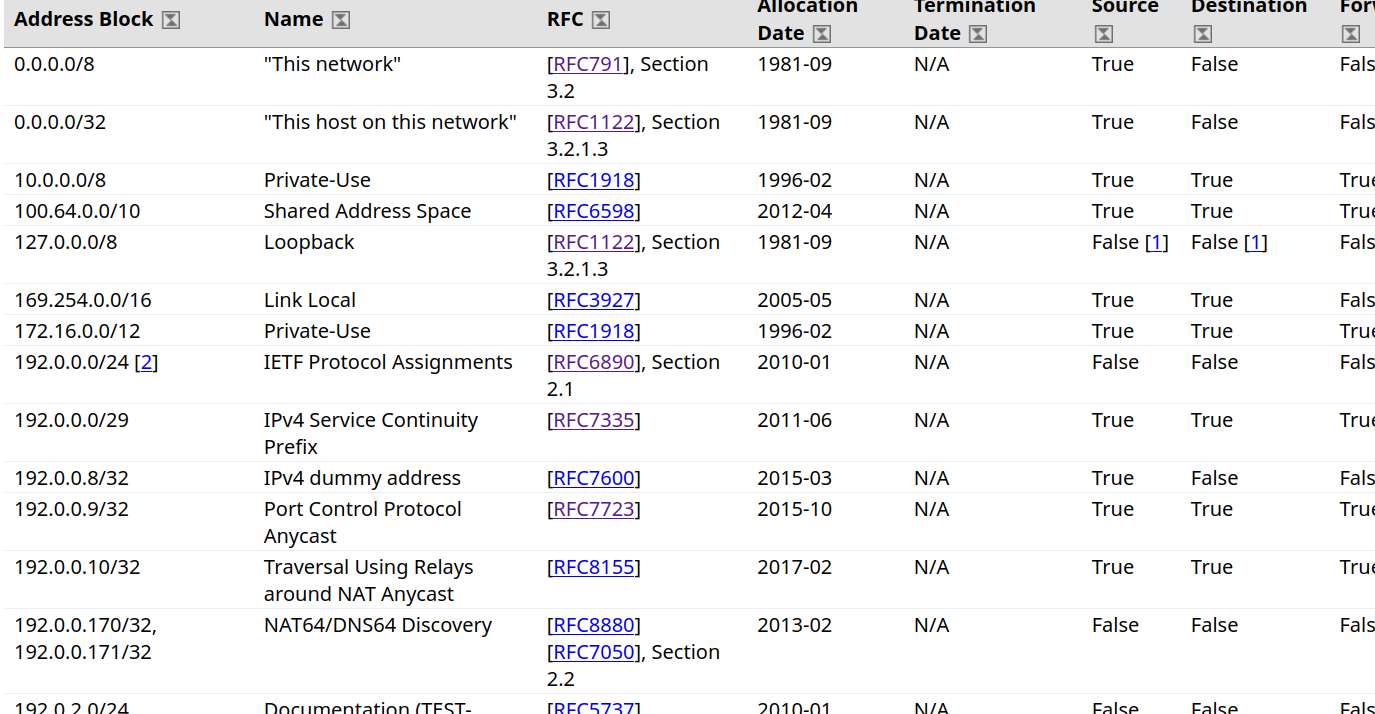
\includegraphics[width=\textwidth]{../arp/iana-special-ipv4-detail}
\end{frame}

\begin{frame}{selected special IP addresses}
\begin{itemize}
\item loopback (current machine) --- {\tt 127/8} (v4), {\tt ::1/128} (v6)
\item link-local (current network only) ---
    \begin{itemize}
    \item {\tt 169.254/16} (v4), {\tt ff80::/10} (v6)
    \end{itemize}
\item private use (non-public networks only) --- \\
    \begin{itemize}
    \item {\tt 192.168/16}, {\tt 172.16/12}, {\tt 10/8} (v4), (kinda) {\tt fc00::/7} (v6)
    \end{itemize}
\item multicast groups and related --- {\tt 224/4} (v4), {\tt ff00::/8} (v6)
    \begin{itemize}
    \item multiple nodes can be part of a single ``multicast group''
    \end{itemize}
\item broadcast (all on current network) --- 
    \begin{itemize}
    \item {\tt 255.255.255.255}, {\tt ff01::1}
    \end{itemize}
\item ``future use'' --- 
    \begin{itemize}
    \item rest of {\tt 240/4} (v4), {\tt 4000::}---{\tt efff::} (v6)
    \end{itemize}
\end{itemize}
\end{frame}
